\label{s:transition-concept}
Starting with a particle attractor as an overview, it is possible to use the attractor to animate the creation and transition of visualisations. Creating marks on a visual representation could be done in two ways:

\begin{enumerate}
\item Each particle tags its spot on the map by leaving an abstract, static mark
\item Each particle moves to its spot on the map and stays
\end{enumerate}

The first method would yield animated creations, with a very basic approach when changing the visual appearance. All particles would draw upcoming visualisations every time, without considering some kind of transition from the first to the second one. The second approach can be used to initially draw the first thematic map when no other visualisation is given. Changing the visual appearance if a thematic map is already shown, the mentioned transition methods can be used.

\begin{figure}[!htb]
\centering
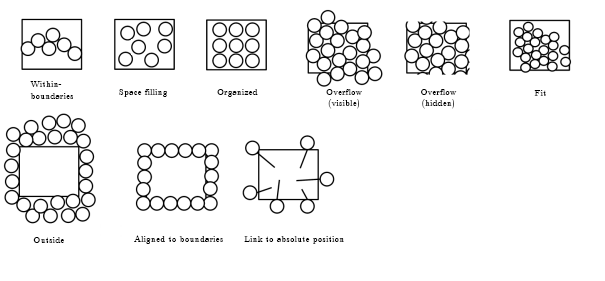
\includegraphics[height=5cm]{images/methods/related/strategies.png}
\caption[
    Particle design strategies to fit in or interact with a perimeter.
]{Particle design strategies to fit in or interact with a perimeter.}
\label{fig:particle-design-strategies}
\end{figure}

Considering the transition from a dot map to any other type of thematic map, the aggregation needs to be animated. Figure \ref{fig:particle-design-strategies} on page \pageref{fig:particle-design-strategies} shows nine different ways of how particles are able to fit in or interact with a perimeter of a given abstract shape. This heavily influences the movement of particles and the readability of the map. Aggregation can not only be done by moving the particle to their new aggregated shape. It could also be accomplished by using the concept of visual sedimentation, but it would also inherit its major weakness. When using the concept of SandDance of building aggregated shapes with units, a map will suffer from overplotting in high-density region, thus leading to visual clutter. Therefore most of the shown unit design strategies will be unusable in combination with certain thematic maps, e.g. proportional symbol maps.

The following list shows some basic concepts of animated transitions. Animating the transition between visual appearances relies on different combinations of the listed transitions. Every transition concept is described with an abbreviation in the list. These abbreviations are used in Chapter \ref{s:animated-transitions-implemented} on page \pageref{s:animated-transitions-implemented} to describe the implemented transitions.

\begin{description}
\item[Area-colour] \hfill \\
Colouring enumeration units where the colour either is determined by the current selected colour scheme or the default colour.

\item[CB-Linear] \hfill \\
Centroid-based linear transition denotes that particles move to their geographical centroid and aggregate after moving. The aggregation can be accomplished with any kind of fitting or interacting with a perimeter.

\item[CB-colour] \hfill \\
Centroid-based colouring is only used in conjunction the \textit{Draw default} and \textit{CB-Linear} transition. Particles moving to its centroid colour their appropriate symbol when reaching the centroid.

\item[Color-Linear] \hfill \\
Color-linear transition can be implemented in two different ways:

\begin{enumerate}
\item Each particle leaves a blur of colour in its area. If more than one particle exists in a certain enumeration unit, the particles blur the area consecutively. Thus each particle increases the color intensity of the enumeration unit.
\item The particles simply fade out and the enumeration units get coloured.
\end{enumerate}

\item[Draw defaults] \hfill \\
Default symbols (circles) are drawn for each enumeration unit at its centroid. Each circle has a default radius. This transition state is mainly used to set up following ones.

\item[Force] \hfill \\
This transition state is only used to create cartograms. Force is dependent on symbols in the screen. It applies collision detection and gravity on those symbols in order to create the Pseudo-Demers cartogram.

\item[Origin-colour] \hfill \\
Origin-colour is the exact opposite of "CB-Colour. All particles are moving from their centroid to their origin location. When leaving their appropriate symbol, the colour of the symbol adapts accordingly.

\item[Scale] \hfill \\
Scaling is also dependent on existing symbols. When scaling is triggered, all symbols are either scaled to their population or back to a default value.

\item[Shape] \hfill \\
This concept of this transition denotes an animation of the shape, for instance morphing a proportional symbol to an enumeration unit is accomplished by a ``Shape''-transition.

\item[Symbol-colour] \hfill \\
All symbols are coloured at once appropriately to their amount of orders.

\item[Symbol-translation] \hfill \\
If the current visualisation is a cartogram and the user wishes to change the visual appearance, all symbols need to move back to their origin again.

\end{description}